
\documentclass[12pt]{article}


\usepackage[T1]{fontenc}
\usepackage[utf8]{inputenc}
\usepackage{amsmath,amssymb}
\usepackage{graphicx}
\usepackage{pgfgantt}
\usepackage[table]{xcolor}
\usepackage{enumitem}

\usepackage[colorlinks=true,allcolors=blue]{hyperref}

\definecolor{Aone}{HTML}{1F4E79}     % dark blue
\definecolor{Atwo}{HTML}{2E75B6}     % medium blue
\definecolor{Athree}{HTML}{9DC3E6}   % light blue

\definecolor{gridgray}{HTML}{E6E6E6}

\newcounter{task}

\newcommand{\taskitem}[2]{%
  \refstepcounter{task}%
  \item[\textbf{T\thetask}\label{#2}] #1
}
\newenvironment{tasks}{
\begin{enumerate}[leftmargin=1.5cm,labelsep=0.5cm,itemsep=.3em]
}{
\end{enumerate}
}
\usepackage[version=4]{mhchem}

\usepackage[
    top=1.7cm,
    bottom=1.7cm,
    left=2cm,
    right=2cm
]{geometry}

\usepackage[
    backend=biber,
    style=authoryear,
    doi=true,
    sorting=nyt,
    maxbibnames=99,
    maxcitenames=2,
    giveninits=true
]{biblatex}

\addbibresource{isotopes.bib}

\setcounter{subsection}{0}
\renewcommand{\thesubsection}{A\arabic{subsection}}

\title{
    \textbf{A closure study to validate a novel isotope-aware
    Lagrangian cloud-microphysics model\\ against airborne measurements}
}

\date{}


\begin{document}
\maketitle
\section{Scientific goal of the project}
Water stable isotopologues are natural tracers of the global hydrological cycle.
Variations in isotopic composition arise from isotopic fractionation accompanying
phase transitions and transport processes in the atmosphere.
Consequently, the isotopic composition of atmospheric water preserves information
about the thermodynamic and microphysical history of clouds
and precipitation.

In atmospheric sciences, the water isotopologues most commonly studied are \ce{HDO},
\ce{H2{}^18O}, and \ce{H2{}^17O}.
Their relative abundances differ from that of the dominant isotopologue \ce{H2{}^16O},
leading to measurable fractionation during evaporation, condensation, and mixing processes.
Recent advances in cavity-enhanced laser spectroscopy have enabled continuous,
high-precision measurements of multiple water isotopologues in atmospheric water vapour,
including triple oxygen isotopes (\ce{^16O}, \ce{^17O}, \ce{^18O}).
The objective is to reconstruct cloud isotopic processes using numerical simulations.
Measurements of the isotopic composition of water vapour below cloud base will be used as boundary
and validation constraints for a particle-resolved cloud model.
The simulated cloud state will subsequently be evaluated against observational data.

A central question is whether isotopic measurements provide sufficient information
to constrain cloud microphysical processes and achieve \emph{isotopic closure} within
a prognostic particle-based framework.
More broadly, it remains unknown whether isotopic closure can be achieved with current
measurement capabilities and advances in particle-based cloud modelling.
If so, an equally important question is what constitutes the minimal mathematical model,
numerical implementation, and observational framework required to achieve it.

In this context, fluctuations in supersaturation play a key role in governing
condensation and evaporation rates at the particle level, thereby influencing
both cloud microphysics and isotopic partitioning.
Recent work has shown that
haze–cloud interactions can be strongly modulated
by supersaturation variability
\parencite{2026_FahandezhSadi_EtAl}.

The project addresses the following research questions:
\begin{enumerate}
    \item[\textbf{Q1}]\label{Q1} Can isotopic closure be achieved in a particle-based
        cloud model using currently available isotopic observations?
    \item[\textbf{Q2}]\label{Q2} Which cloud microphysical processes leave
        identifiable signatures in the isotopic composition
        of atmospheric water?
    \item[\textbf{Q3}]\label{Q3} To what extent do isotopic measurements constrain
        key cloud properties such as supersaturation variability,
        phase partitioning, and mixing?
    \item[\textbf{Q4}]\label{Q4} What is the minimal physical and numerical
        framework required to achieve isotopic closure
        while maintaining predictive skill?
\end{enumerate}


\section{Significance of the project}
Cloud microphysical processes remain one of the largest sources of
uncertainty in weather prediction and climate projections \parencite{IPCC2021_WGI}.
Processes such as condensation, evaporation, entrainment,
and phase transitions between vapour, liquid, and ice strongly
influence cloud lifetime, precipitation formation,
and radiative properties.
Yet many of these processes cannot
be directly observed and therefore remain poorly constrained
in atmospheric models \parencite{2013_Grabowski_Wang}.

Stable water isotopologues provide a unique observational tracer 
of cloud evolution.
During phase transitions, isotopic fractionation modifies
the relative abundance of isotopologues in vapour, liquid, and ice \parencite{2017_Lamb_EtAl}.
Consequently, isotopic composition contains information about 
the thermodynamic and microphysical history of air masses and
clouds \parencite{2013_Bolot_EtAl}.

Theoretical descriptions of equilibrium and kinetic isotopic
fractionation are well established,
and stable water isotopologues are routinely represented
in global and regional atmospheric models \parencite{2016_Galewsky_EtAl}.
These isotope-enabled models have significantly improved
understanding of large-scale moisture transport and
the atmospheric hydrological cycle \parencite{2020_Risi_EtAl}.
However, most existing approaches rely on Eulerian formulations
and bulk cloud parameterisations, limiting their ability
to resolve the particle-scale processes responsible for
generating isotopic signatures \parencite{1984_Joussaume_EtAl, 2008_Yoshimura_EtAl, 2011_Werner_EtAl, 2016_Galewsky_EtAl}.


At the same time, particle-based cloud models have emerged 
as a state-of-the-art framework for studying cloud microphysics \parencite{2009_Shima_EtAl}.
By explicitly representing aerosol particles, cloud droplets,
and ice particles, these models provide detailed descriptions of condensation,
evaporation, freezing, and other microphysical processes.

Despite these advances, isotopic composition has rarely been 
considered within particle-based cloud modelling,
and its potential as a constraint on cloud evolution remains
largely unexplored.
A~fundamental unresolved question is whether isotopic observations
contain sufficient information to constrain cloud microphysical
processes and achieve isotopic closure.
Analogously to cloud condensation nuclei closure studies,
isotopic closure can be understood as the ability to consistently explain observed
isotopic composition using a physically based description of cloud evolution \parencite{2021_Knopf_EtAla}.
While isotopic measurements are increasingly available and
process-resolving cloud models are becoming increasingly sophisticated,
no systematic framework currently exists for assessing isotopic
closure in cloud systems.

The proposed project addresses this gap by investigating isotopic
closure using particle-based cloud simulations and isotopic observations
from in-cloud measurements and laboratory experiments.
The project is pioneering because it introduces isotopic closure
as a research objective in cloud physics and establishes
a link between isotope-enabled observations and modern cloud microphysics.
The results will provide insight into the information content
of isotopic measurements, improve understanding of isotopic signatures
generated by cloud processes, and contribute to the development
of new observational constraints for atmospheric modelling.

\section{Research Concept and Work Plan}
The project is divided into three areas: development of a physically
consistent theoretical description of isotopic fractionation in cloud microphysical
processes (\ref{A1}),
its implementation in a particle-based cloud microphysics framework (\ref{A2}),
and evaluation against observational and laboratory data (\ref{A3}).
Feedback between these components ensures continuous refinement
of both model formulation and interpretation of isotopic signals.

The proposed research builds on preliminary results obtained
within a previous NCN project, in which the PI contributed to early development
of isotope-enabled particle-based cloud modelling within the Super-Droplet Method framework.
The preliminary results (PR) are described in each relevant research area (A1--A3)
and provide a proof-of-concept for prognostic isotopic tracking in Lagrangian cloud microphysics.

\subsection{Theory: isotopic cloud microphysics}\label{A1}
This research area focuses on developing a unified theoretical framework for
isotopic fractionation in liquid–vapour systems,
with a conceptual extension to ice-phase processes.
The objective is to formulate governing equations that
describe isotope-specific mass transfer in
cloud environments, including both equilibrium and kinetic processes.
The~analysis will include:
(i) derivation of isotopic mass balance equations for vapour, liquid, and ice
phases,
(ii) identification of limiting regimes such as equilibrium fractionation and
Rayleigh-type distillation,
and (iii) formulation of dimensionless control parameters, including the Bolin
number introduced in preliminary studies.

A key objective is to identify the minimal set of physically
essential processes that govern isotopic signatures in clouds.
This includes condensation, evaporation, deposition, sublimation,
and freezing, expressed in a~form consistent with particle-based modelling.
The outcome of~\ref{A1} is a~closed and consistent theoretical description
of isotopic cloud microphysics suitable for numerical implementation.

In addition to model validation, the proposed framework includes
a~systematic analysis of numerical model errors,
sensitivity to key physical parameters,
and uncertainty propagation within the isotopic closure framework. 
This encompasses both local sensitivity analysis of governing 
equations and global sensitivity studies based on numerical experiments.
Uncertainty propagation will be quantified through ensemble simulations,
allowing assessment of how uncertainties in microphysical parameters,
initial conditions, and isotopic boundary conditions influence
the simulated isotopic composition.
Particular attention will be given to distinguishing
structural model uncertainty from observational uncertainty.


\subsubsection*{Preliminary results}
A dimensionless framework for describing the evolution of isotopic composition of water in particle-based
cloud models was introduced through the concept of the Bolin number.
The formulation builds on the original work of \textcite{1958_Bolin}, developed for tritium transport in atmospheric water.

The Bolin number expresses the relative importance of diffusive and phase-change-driven isotopic exchange between isotopologues. It is defined as:
$\textbf{Bo} = \frac{\tau_\text{heavy}}{\tau_\text{light}}$,
where $\tau = \left(\frac{1}{m} \frac{dm}{dt}\right)^{-1}$
is the characteristic equilibration timescale of a given isotopologue,
and $m$ denotes its mass in a droplet.

By defining this number explicitly, the evolution of a heavy isotopologue can be inferred from the dynamics of the corresponding light isotopologue (or approximately from the total droplet mass).
The Bolin number provides a compact representation of isotopic exchange efficiency, incorporating equilibrium fractionation ($\alpha_\text{eq}$),
diffusive transport (including ventilation effects), and environmental controls such as temperature and saturation ratio.
This formulation captures both equilibrium and kinetic fractionation regimes within a unified dimensionless framework.

The Bolin number was validated against equilibrium isotopic fractionation curves for water vapour and liquid phases reported by \textcite{1994_Gedzelman_Arnold}.
The comparison is shown in Fig.~\ref{fig:bolin},
where colors denote values predicted by the Bolin-number-based formulation,
while black lines reproduce the equilibrium regimes for liquid ($S^\text{eq}_\text{liquid}$)
and vapour ($S^\text{eq}_\text{vapour}$) from \textcite{1994_Gedzelman_Arnold}.

\begin{figure}[h]
    \centering
    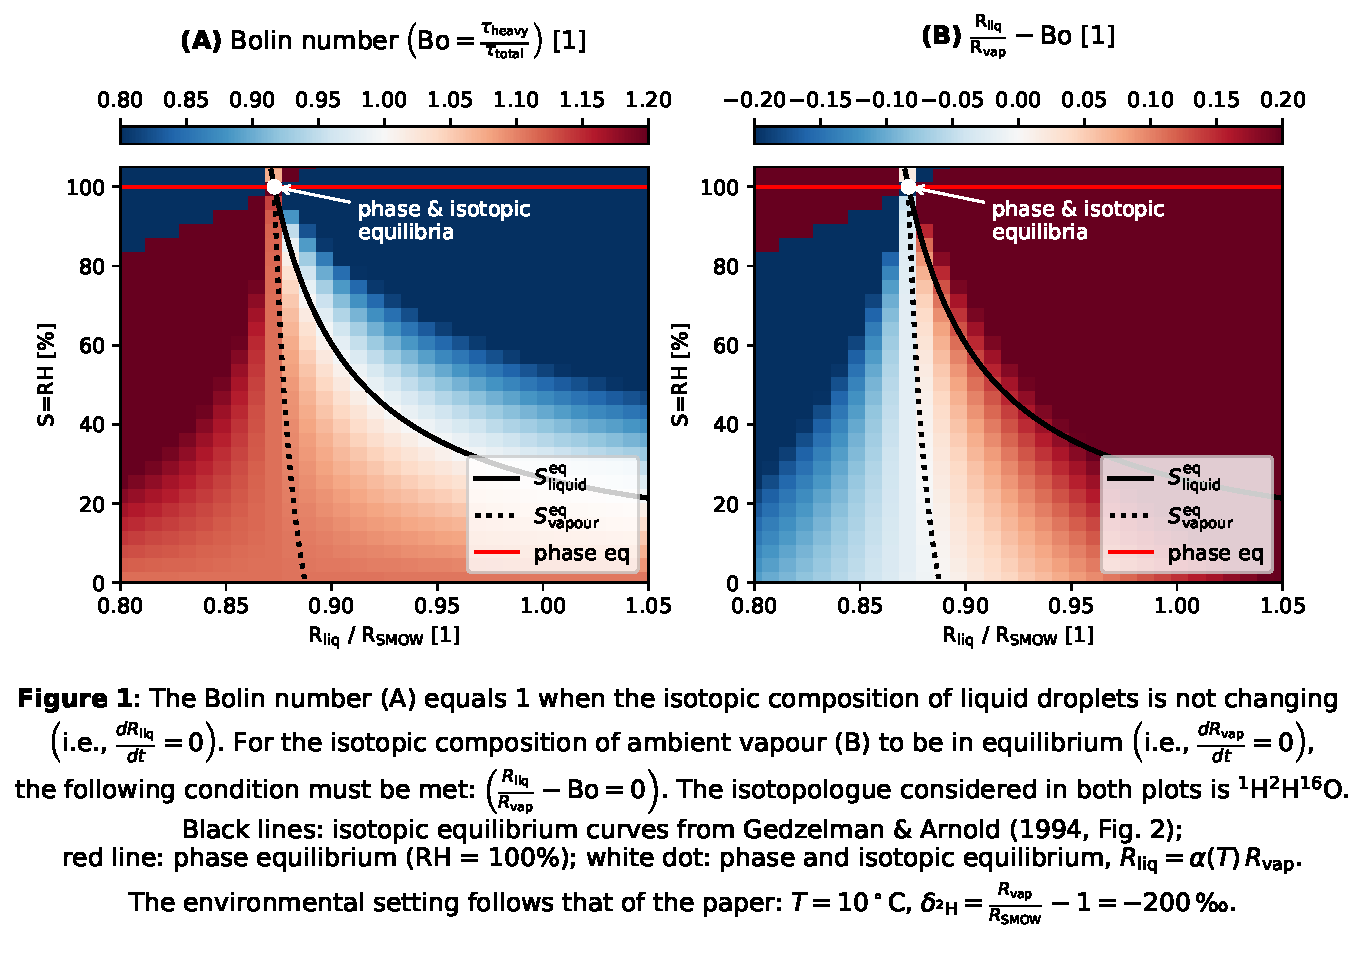
\includegraphics[width=.9\textwidth]{Bo} 
    \caption{Conditions for isotopic steady state in liquid droplets (A)
        and ambient vapour (B).
        Panel A~shows the locus where the isotopic composition
        of cloud droplets remains constant ($\left(dR_{\mathrm{liq}}/dt=0\right)$),
        corresponding to ($\mathrm{Bo}=1$).
        Panel B shows the locus where the isotopic composition of vapour
        remains constant ($\left(dR_{\mathrm{vap}}/dt=0\right)$),
        corresponding to ($R_{\mathrm{liq}}/R_{\mathrm{vap}}-\mathrm{Bo}=0$).
        The figure illustrates the theoretical equilibrium relationships governing
        isotopic exchange between liquid and vapour phases. 
        The isotopologue considered is (\ce{HDO}).
        Black lines indicate isotopic equilibrium curves, the red line phase equilibrium (RH = 100$\%$),
        and the white dot simultaneous phase and isotopic equilibrium.
}
    \label{fig:bolin}
\end{figure}
The developed concept has been accepted for presentation at the 17th Conference
on Cloud Physics (AMS Madison Summit 2026).


\subsection{Numerics: particle-based implementation
    and simulation framework}\label{A2}

This research area focuses on implementing the proposed theoretical
framework within the particle-based cloud microphysics model PySDM,
which is based on the Super-Droplet Method (SDM) \parencite{2009_Shima_EtAl}.

\subsubsection*{State of the art}
The Super-Droplet Method (SDM) is a particle-based Lagrangian cloud microphysics framework 
in which cloud and aerosol populations are represented by computational particles 
(super-droplets) carrying multiplicities \parencite{2009_Shima_EtAl}.

PySDM is an open-source implementation of SDM that enables simulations of cloud
microphysical processes such as condensation, evaporation, collision–coalescence,
and ice-phase transformations in box, parcel, and single-column configurations
\parencite{2022_Bartman_EtAl, 2023_DeJong_EtAl}.
Its particle-based structure allows straightforward extension with additional prognostic
variables, such as isotopic composition.

\subsubsection*{Preliminary results}

The PI has implemented isotopic evolution of water vapour
and cloud droplets for a single heavy isotopologue 
within the PySDM framework based on the Super-Droplet Method.
This extension of PySDM enables prognostic isotopic composition of
individual computational particles,
allowing explicit representation of isotopic fractionation during
cloud microphysical processes.

\subsubsection*{Planned work}
Building on the existing conceptual formulation,
the model will be implemented within PySDM by extending the current single-isotopologue
treatment to a fully mixed-phase, multi-isotopologue framework.
At present, isotopic tracking has only been developed for vapour and liquid phases;
representation of isotopes in the ice phase remains to be implemented.
The proposed work will therefore generalise the formulation to include
prognostic isotopic composition in all three phases and enable consistent
treatment of fractionation during phase transitions, diffusive exchange,
and collisional processes within a particle-resolved framework.

The numerical implementation will be verified using conservation diagnostics
and comparison against analytical limiting cases.
After implementation, the model will be explored in idealised numerical
experiments (box, parcel, and column configurations) to quantify sensitivity
of isotopic composition to key microphysical and environmental controls,
including supersaturation, temperature, droplet size distribution, and ice fraction.

The outcome will be a fully mixed-phase, isotope-enabled PySDM extension
suitable for subsequent application to cloud process studies.

\subsection{Data: observational and experimental validation}\label{A3}
This research area is dedicated to assessing model predictions through
comparison with observational and experimental data.
The model will be tested using isotopic measurements from aircraft campaigns,
including the CAESAR dataset, as well as laboratory experiments
performed in collaboration with NSF NCAR (Elise Rosky).
Together, these datasets offer complementary constraints spanning vapour,
cloud water, ice, and precipitation phases.

The laboratory component is currently in a~preliminary stage,
and its design will evolve in parallel with the development
of the modelling framework.
This co-development approach highlights the potential and scientific
importance of the proposed project,
as it enables direct feedback between numerical modelling
and experimental design.
It also ensures consistency between observational capabilities,
experimental constraints, and the evolving requirements of the analysis,
while supporting close interdisciplinary collaboration.

The analysis will focus on three aspects:
(i) agreement between simulated and observed isotopic composition,
(ii) sensitivity of isotopic signals to cloud microphysical processes, and
(iii) ability of isotopic measurements to constrain cloud evolution and assess
closure.
The outcome of~\ref{A3} is an empirical evaluation of isotopic closure and a
quantification of the information content of isotopic observations in
mixed-phase cloud systems.

\subsection*{Data availability}
The CAESAR field campaign provides an openly accessible dataset of cold-air outbreak
clouds over the Nordic Seas (EOL archive).
Collaboration with Elise Rosky was initiated during the PI's visit to NSF NCAR in 2025.
As an outcome of this collaboration, the PI contributed to a conference abstract
presented by Dr. Rosky at the AGU Fall Meeting 2025 on isotopic observations
from the CAESAR campaign \parencite{2025_Rosky_MixedPhaseIsotopes}.
The dataset will serve as one of the observational benchmarks
for model evaluation within the proposed project.


\subsection*{Integration of A1--A3}
The three research areas are strongly coupled.
\ref{A1} defines the physical
description of isotopic processes,
\ref{A2} translates this description into a
numerical particle-based framework,
and~\ref{A3}
provides observational constraints and evaluates model performance
against measurements and laboratory data.
This integrated structure enables a~systematic investigation of isotopic
closure, ensuring consistency between theory, numerical representation, and
observational evidence.


\section{Project Tasks, Milestones and Schedule}
The task structure follows the three research areas defined in the project concept (\ref{A1}, \ref{A2}, \ref{A3}),
ensuring consistency between theoretical development,
numerical implementation, and data-driven evaluation.
This structure supports iterative feedback between model formulation
and physical interpretation of isotopic signals.

The research plan is formulated according to
the SMART principle (specific, measurable, achievable, relevant, and time-bound).
Each work package is decomposed into specific tasks.




\subsection*{Tasks}

The project consists of core tasks structured into three work packages:
theoretical development, numerical implementation, and observational validation.
Each task produces at least one major research output (peer-reviewed publication
and/or open-source software release).

% ==========================================================
\subsection{Theory: Isotopic Cloud Microphysics}

\begin{tasks}

\taskitem
{Derive a closed set of governing equations for isotope-resolved mass transfer
between vapour, liquid, and ice phases in mixed-phase clouds. The formulation
includes equilibrium fractionation, kinetic effects, and phase-change-driven
non-equilibrium processes in a particle-based framework.}
{task:T1}

\textbf{Deliverable:} Results presented on EGU General Assembly (Months 6--12).

\vspace{0.5em}

\taskitem
{Identify limiting regimes of isotope evolution (equilibrium, Rayleigh
distillation, diffusion-limited growth) and construct reduced-order models.
Develop a regime map of isotopic behaviour and sensitivity structure.}
{task:T2}

\textbf{Deliverables:}
(i) reduced-order model suite with validity regimes clearly defined,  
(ii) diagnostic criteria for isotopic closure breakdown. 

\textbf{Dissemination:} Conference poster/talk (EGU) (Months 12--18).

\vspace{0.4em}

\taskitem
{Quantify sensitivity of isotopic composition to microphysical parameters
and atmospheric forcing using local and global sensitivity analysis,
and construct an uncertainty propagation framework linking parameter
uncertainty to isotopic observables.}
{task:T3}

\textbf{Deliverables:}
(i) ensemble-based uncertainty quantification framework, 
(ii) reproducible analysis notebooks.

\textbf{Dissemination:} ICCP / EGU presentation (Months 18--24).
    
\end{tasks}

% ==========================================================
\subsection{Numerical Framework: Particle-Based Implementation}

\begin{tasks}

\taskitem
{Implement isotope-resolved cloud microphysics in the PySDM framework,
including vapour, liquid, and ice phases. Ensure mass conservation,
thermodynamic consistency, and validation against analytical limiting cases.}
{task:T4}

\textbf{Deliverable:}
Open-source PySDM isotope module (Zenodo DOI + GitHub release).

\textbf{Dissemination:} EGU demo (Months 12--18).

\vspace{0.5em}

\taskitem
{Develop a minimal isotope-enabled cloud model for controlled numerical
experiments. The framework isolates key processes controlling isotopic closure,
including supersaturation variability, mixing, and phase partitioning.}
{task:T5}

    \textbf{Deliverables:}
    (i) full mixed-phase isotope-enabled PySDM extension,  
    (ii) verification against analytical fractionation limits,  
    (iii) documented API for isotopic particle attributes.
    
    \textbf{Dissemination:}
    Summer school/tutorial release (Months 14--20).

\end{tasks}

% ==========================================================
\subsection{Validation and Closure Assessment}

\begin{tasks}

    \taskitem
    {Construct and preprocess observational and laboratory datasets (CAESAR,
    NCAR experiments), including uncertainty characterization and mapping to model
    state variables.}
    {task:T6}
    
    \textbf{Deliverable:}
    Curated, model-ready dataset + preprocessing pipeline.

\vspace{0.5em}

\taskitem
    {Perform model–observation comparison and evaluate isotopic closure.
    Identify which microphysical processes are required to reproduce observed
    isotopic signatures and quantify closure regimes.}
    {task:T7}
    
    \textbf{Deliverables:}
    (i) formal closure assessment framework,  
    (ii) classification of closure regimes (closed / partially constrained / unconstrained).

    \textbf{Dissemination:} Peer-reviewed paper on isotope closure,      
    final open-source release of full framework (model + diagnostics + datasets) (Months 18--24).
    
\end{tasks}

% ==========================================================
\subsection*{Milestones}

\begin{itemize}

\item[\textbf{M1}] Completion of theoretical framework for isotope-resolved cloud microphysics
and identification of governing equations (Month 12).

\item[\textbf{M2}] Completion of numerical implementation in PySDM and validation of isotope tracking
in idealised simulations (Month 18).

\item[\textbf{M3}] Integration of observational and laboratory datasets with model framework
and initiation of systematic evaluation (Month 12).

\item[\textbf{M4}] Completion of isotopic closure assessment and identification of minimal physical
requirements for closure (Month 24).

\end{itemize}

% ==========================================================
\subsection*{Schedule}

The project is structured over 24 months with strong feedback between theory,
numerics, and data analysis. Dataset preparation starts early, while closure
analysis is performed in the final phase.


\begin{figure}[t]
\centering
\footnotesize
\begin{ganttchart}[
    hgrid,
    vgrid,
    hgrid style/.style={draw=gridgray, line width=0.3pt},
    vgrid style/.style={draw=gridgray, line width=0.3pt},
    x unit=0.55cm,
    y unit chart=0.55cm,
    bar height=0.7,
    group height=0.8,
    milestone height=0.7,
    progress label text={},
]{1}{24}

\ganttset{
group/.style={
    draw=Aone,
    fill=Aone!20,
    line width=0.6pt
}
}

\gantttitle{Project Duration (Months)}{24} \\
\gantttitlelist{1,...,24}{1} \\

% ===================== A1 THEORY =====================
\ganttset{
bar/.style={
    fill=Aone,
    draw=Aone,
    line width=0.4pt
}
}

\ganttgroup{\ref{A1} Theory}{1}{18} \\

\ganttbar{Task \ref{task:T1}}{1}{8} \\
\ganttbar{Task \ref{task:T2}}{4}{12} \\
\ganttbar{Task \ref{task:T3}}{10}{18} \\

\ganttmilestone{M1 Theory framework}{12} \\

% ===================== A2 NUMERICS =====================
\ganttset{
bar/.style={
    fill=Atwo,
    draw=Atwo,
    line width=0.4pt
}
}

\ganttgroup{\ref{A2} Numerics}{4}{18} \\

\ganttbar{Task \ref{task:T4}}{4}{12} \\
\ganttbar{Task \ref{task:T5}}{10}{18} \\

\ganttmilestone{M2 Numerical framework}{18} \\

% ===================== A3 VALIDATION =====================
\ganttset{
bar/.style={
    fill=Athree,
    draw=Athree,
    line width=0.4pt
}
}

\ganttgroup{\ref{A3} Data}{5}{24} \\

\ganttbar{Task \ref{task:T6}}{5}{12} \\
\ganttbar{Task \ref{task:T7}}{10}{24} \\

\ganttmilestone{M3 Data integration}{12} \\
\ganttmilestone{M4 Closure assessment}{24}

\end{ganttchart}

\caption{
Project timeline structured into three work packages:
\ref{A1}, \ref{A2}, and \ref{A3}.
}
\label{fig:gantt}
\end{figure}

\subsection*{Result dissemination}
Project results will be disseminated through peer-reviewed publication,
conference presentations, research visits, and open-source software releases.
Results will be submitted to international journal relevant to atmospheric
modelling and isotope hydrology.
Journals taken into account: \emph{Tellus B: Chemical and Physical
Meteorology},
\emph{Journal of Advances in Modeling Earth Systems}, and
\emph{Geoscientific Model Development}.
Interim and final results will be presented as talks or posters at
international conferences, including the European Geosciences Union General
Assembly and the International Conference on Clouds and Precipitation.

The project includes a~research visit to the United States, a~visit of an
international collaborator to AGH University of Krakow, and participation of the MSc
student in an international summer school.
All software developed within the project will be released as open source via
GitHub, accompanied by documentation and reproducible Jupyter notebooks
demonstrating the proposed methods and numerical experiments.
Data-processing
workflows required to reproduce published results will be made publicly
available.


\section{Research methodology}
Underlying scientific methodology, methods, techniques and research tools,
methods of results analysis, and equipment used in the research are based 
on a~combination of physically based modelling, particle-based numerical simulation,
and systematic data-model comparison.

\subsection*{PySDM-based modelling framework}
The numerical core of the model is the PySDM implementation of the Super-Droplet Method (SDM),
which is used as the Lagrangian particle-resolved framework 
for cloud microphysics in this project.
In this work, PySDM is extended by augmenting each super-droplet with prognostic variables
describing the isotopic composition of water in vapour, liquid, and ice phases.
This preserves the original SDM structure while enabling simulation of isotope-resolved
cloud microphysics.
The resulting framework is used for idealised box, parcel, and column simulations
to study isotope–microphysics interactions under controlled conditions.

\subsection*{Jupyter notebook–based simulation and analysis environment}
A central component of the project is the use of Jupyter notebooks
as the primary interface for model development, numerical experiments,
and data analysis.
Each notebook constitutes a fully self-contained and executable
research workflow, including (i) model configuration and initialization,
(ii) simulation execution,
(iii) post-processing and diagnostics, and 
(iv) visualisation of results.
This design ensures that every numerical experiment is fully reproducible
and can be independently executed without additional external
scripts or hidden dependencies.

Notebooks function simultaneously as an executable research workflow, a documentation format,  
and a reproducible dissemination layer for scientific results.
Within this project, notebooks are integrated with version control
and continuous integration (CI) pipelines. 
This ensures that all simulations remain reproducible
over time and that changes in the codebase automatically trigger 
validation of numerical correctness.

\subsection*{Reproducibility, software engineering, and research workflow}
The project follows established reproducible research practices.
All components of the modelling system, including PySDM extensions,
simulation configurations, and analysis notebooks,
are managed in version-controlled repositories and continuously
validated through automated CI pipelines.
The CI system performs unit tests verifying physical consistency (e.g. mass conservation and isotopic bounds),
regression tests ensuring numerical stability,
and benchmark tests against analytical or well-established reference solutions.
This workflow ensures that model development remains transparent, 
scientifically traceable, and computationally robust.

\subsection*{Educational and training component}
The Jupyter-based workflow plays a key role in the training component
of the project.
The MSc/Erasmus+/PhD student involved in the project will
contribute directly to the development of simulation notebooks, including
simplified educational model configurations,
reproducible experiment templates for key processes,
and interactive visualisation and analysis tools.

This approach lowers the entry barrier to particle-based
cloud microphysics and provides hands-on training in modern
scientific computing, including numerical modelling,
uncertainty quantification, and reproducible research practices.
As a result, the project integrates scientific development
with structured training in computational atmospheric physics.

\section*{Composition and qualifications of the research team}
The research team consists of the Principal Investigator (PI),
a scientific mentor, and one student, 
forming a compact group focused on particle-based cloud microphysics
and isotope-enabled modelling.
\\

\noindent\textbf{Principal Investigator}
The Principal Investigator is a PhD student in the physical
sciences with a background in mathematics and numerical modelling. 
The PI has experience in scientific computing and Python-based development,
with a focus on particle-based atmospheric simulation frameworks.
The PI is the main developer of the isotope-enabled cloud microphysics
framework presented in this proposal, integrating theoretical 
formulations, numerical implementation, and data analysis within
a unified modelling environment.
Previous work includes isotope-enabled cloud modelling 
and international collaboration at 
the National Center for Atmospheric Research (NCAR), 
including work with Dr. Elise Rosky on mixed-phase cloud isotopic processes.
\\

\noindent\textbf{Scientific mentor}
The scientific mentor is Dr. Sylwester Arabas,
co-developer of the PySDM particle-based cloud microphysics 
framework and an expert in Lagrangian cloud modelling and 
scientific computing.
The mentor contributes to the development of open-source
atmospheric modelling tools and ensures the physical and numerical 
robustness of the SDM-based framework.
\\

\noindent\textbf{Student contribution}
The student (MSc/Erasmus+/PhD level) will support development
of a~minimal computational environment for isotope-enabled cloud simulations.
The implementation will be in Python (optionally Julia) and will 
serve as a reusable and accessible framework for research and training
in cloud microphysics.
\\

\noindent\textbf{Environmental Physics group background}
The PI and scientific mentor are affiliated with the
Environmental Physics group, which conducts research on atmospheric
isotope systematics and tracer-based hydrological processes.
The group has experience in the measurement, analysis,
and interpretation of stable water isotopes in environmental
and atmospheric applications, including diffusion and phase-change
fractionation processes \parencite{2022_Pierchala_EtAl}.
This background supports the integration of isotope observations
with particle-based cloud modelling and provides methodological 
continuity between observational and numerical approaches.

\appendix

\clearpage
\pagenumbering{gobble}
\printbibliography
\end{document}